\chapter[Introdução]{Introdução}

Ao longo dos anos, agricultores buscaram soluções para o cultivo em ambientes protegidos e seguros. Além disso, houve uma necessidade de produzir em períodos climáticos desfavoráveis, ter o melhor controle do plantio como um todo e realizar o desuso quanto aos agrotóxicos causadores de enfermos. Essas causas, inspirou a realização de muito estudo para proteger o plantio dos dados causados pela natureza e para a não utilização de pesticidas, sendo estes responsáveis por doenças em consumidores. Motivou-se então a criação de um microclima adequado para o cultivo do plantio e tornar o desenvolvimento de hortaliças mais seguro e controlável. 

\section{Contexto}
 
Um grupos de alunos de Engenharia da Universidade de Brasília do Campus do Gama propuseram desenvolver uma estufa hidropônica automatizada, nomeada como Greenhouse, capaz de manter as condições ideais para o cultivo de hortaliças, onde há a permissão do uso de configurações pré-definidas quanto a customização das condições internas, tendo então a disponibilidade do fornecimento de dados ao usuário através de uma interface local, um aplicativo mobile e um sistema
web. O escopo não engloba a produção de plantas que não sejam hortaliças; a produção de hortaliças que não suportam um sistema de hidroponia; o controle da umidade; e a utilização em um ambiente aberto (i.e. outdoor). 

\section{Justificativa}

O objetivo do projeto Greenhouse é fornecer a moradores de casas e apartamentos uma forma automatizada de cultivar hortaliças em suas residências. Isto irá permitir que, mesmo sem uma grande área dedicada, tempo, ou conhecimentos sobre cultivo, os usuários possam cultivar seus próprios produtos orgânicos para consumo próprio.

\section{Escopo do projeto}
 \subsection{Premissas}
  
 \begin{itemize}
 	\item  O produto será utilizado exclusivamente para o cultivo de hortaliças.
 	\item O produto será utilizado exclusivamente em um ambiente fechado (i.e. não será utilizado ao ar livre).
 	\item  O produto estará conectado a uma fonte de água.
 	\item Não serão utilizados pesticidas nas hortaliças cultivadas no produto, ou na água utilizada pelo mesmo.
 \end{itemize}
  
  \subsection{Restrições}
  
  \begin{itemize}
  	\item Irá controlar uma situação de um sistema especificamente hidropônico.
  	\item O produto não poderá ser instalado em um sistema aberto (i.e. outdoor).
  \end{itemize}
                             
  \subsection{Mapeamento do modelo 5W2H}
  O projeto foi mapeado utilizando o modelo 5W2H, descrito a seguir.
	  \subsubsection{What - O quê?}
	  
		\begin{itemize}
			
			\item Um Plantário estufa automatizada.
			
		\end{itemize}
	
	  \subsubsection{Why - Por quê?}
	  
	 	\begin{itemize}
	 		
	  		\item Facilitar e incentivar o cultivo caseiro.
	  		
	  		\item Reduzir gastos com hortaliças.
	  		
	  		\item Otimizar a utilização de espaço para cultivo.
	  		
	  	\end{itemize}
  	
  	\subsubsection{Where - Onde?}
  	
  	\begin{itemize}
  		
  		\item Na UnB/FGA.
  		
  		\item No Galpão da UnB/FGA.
  		
  		\item Na residência de um ou mais membros.
  		
  	\end{itemize}
  
	\subsubsection{Who - Quem?}
	
	\begin{itemize}
		
		\item Alunos dos cursos de Engenharia de Software, Engenharia Aeroespacial, Engenharia Eletrônica, Engenharia Automotiva e Engenharia de Energia da UnB/FGA.
		
	\end{itemize}

	\subsubsection{How - Como?}
	
	\begin{itemize}
		
		\item Por meio de pesquisas e pelos conhecimentos prévios dos membros da equipe de projeto com a orientação dos professores da disciplina de Projeto Integrador.
		
	\end{itemize}

	\subsubsection{How Much - Quanto?}
	
	\begin{itemize}
		
		\item O detalhamento dos custos do projeto pode ser visto na tabela 2.
		
	\end{itemize}
  	
\section{Detalhamento do escopo}

\subsection{Projeto}
A equipe Greenhouse pretende contornar as adversidades descritas ao realizar um controle do cultivo, ao constatar a praticidade e despreocupação do usuário final com relação ao desenvolvimento automatizado das hortaliças, além do controle do usuário para as mudanças pertinentes de cada espécie, notificando-o sempre que necessário para que o mesmo esteja ciente do monitoramento do plantio.

O público alvo do projeto são as pessoas preocupadas em produzir o cultivo de hortaliças em um local protegido e em fácil acesso, monitoramento e controle de seu equipamento, sendo este instalado em uma casa, apartamento ou em qualquer local que forneça suas especificações de dimensionamento e que tenha conexão a uma fonte de água.

\subsection{Produto}

O sistema de automatização da estufa irá controlar a temperatura e umidade interna, realizar a abertura automática da gaveta onde se comportará o sistema composto pelas hortaliças e monitorar nível da água, temperatura da água e pH da água.

O sistema funcionará da seguinte forma: o usuário prepara os sachês com substâncias específicas para a germinação, implementa a semente da hortaliça de acordo com as especificações ideais de plantio, informa no sistema web a espécie da hortaliça e acompanha o desenvolvimento da mesma por meio de gráficos e informações de uso disponíveis no sistema web, pois os dados coletados pelos sensores da estufa irá para o servidor web e estará disponível para o monitoramento de todos os dados previamente planejados e o controle de alguns dados específicos, caso não há internet no local de instalação da estufa, os dados estarão empilhados e disponíveis para o acompanhamento quando houver conexão de internet.

A estrutura completa terá dimensões ideias para sua instalação em apartamentos, casas e afins.
\section{Objetivos}

\subsection{Objetivo Geral}

Levando em consideração a dificuldade das pessoas em produzir hortaliças por meio do cultivo residencial, principalmente aquelas que convivem em residências privadas de luz solar e jardinagem, o deferido trabalho propõe a criação de uma estufa hidropônica automatizada dando importância nos aspectos agronômicos para que seja cultivado hortaliças sem dificuldades e que seja realizada a transparência do usuário com relação ao monitoramento e o controle de alguns parâmetros relavantes para o desenvolvimento das hortaliças. 

\subsection{Objetivos Específicos}

A partir das diretrizes acima, o presente trabalho determina que seja desenvolvido os seguintes quesitos a serem desenvolvidos:
	
	\begin{itemize}
 		
 		\item Produzir uma estrutura composta por um chassi externo isolado que irá conter uma área de cultivo, uma área do reservatório e uma área de iluminação.
 		
 		\item Realizar a comunicação com o sensor DHT22 para umidade relativa do ar e temperatura do ar.
 		
 		\item Realizar a comunicação com o sensor DS18B20 para temperatura da água.
 		
 		\item Realizar a comunicação com o sensor PCF8591 para leitura do PH e Luminosidade a partir de um Conversor A/D.
 		
 		\item Realizar a comunicação d sensores de nível de água por meio de boias.
 		
 		\item A comunicação entre os sensores se torna necessário para o monitoramento dos parâmetros pertinentes.
 		
 		\item Projetar e implementar um sistema que irá realizar a coleta e envio de dados para uma plataforma Web e Mobile por meio de uma Rapberry Pi.
 		
 		\item Projetar e implementar um sistema Web e Mobile.
 		
 		\item Manter um ambiente ideal para o cultivo de diversas hortaliças.
 		
 		\item Otimizar condições internas da estufa para cultivos específicos a partir de um banco de dados
 		
	\end{itemize}

\section{Metodologia de gerenciamento}

Em decorrência do presente trabalho propor em planejar e produzir uma estufa hidropônica automatizada, há uma necessidade de utilizar uma metodologia específica para o gerenciamento do projeto como um todo, para que o planejamento do trabalho seja guiado na forma previamente produzida.

Sendo assim, a equipe irá utilizar a metodologia ágil, mais especificamente o SCRUM, sendo este responsável pela agregação eficiente do valor ao cliente, atrelado ao modelo do Guia PMBOK® que irá realizar toda a estrutura de gerenciamento de projeto para as áreas de conhecimento requisitadas na construção do projeto.

Os seguintes planos de gerenciamento serão produzidos para a construção do projeto:

\begin{itemize}
	
	\item Plano de gerenciamento de tempo: Área que irá definir as atividades específicas do projeto, onde se estima a duração de cada atividade e onde as colocam em sequência cronológica, ao final é gerado um cronograma que ilustra todas as atividades e as datas de resolução das mesmas.
	
	\item Plano de gerenciamento de custos: Área que determina informações acerca das estimativas, orçamentos e controle dos custos do projeto, de modo que o projeto seja realizado dentro do orçamento estipulado.
	
	\item Plano de gerenciamento de riscos: Busca descrever os riscos que podem afetar o projeto, e realiza é realizado uma análise quantitativa e qualitativa do dos riscos.
	
	\item Plano de gerenciamento de comunicação: Área responsável por selecionar ferramentas de comunicação, definir um meio de comunicação que envolva todos os membros da equipe e agregar valor ao projeto por meio da intercomunicação dos stakeholders.
	
	\item Plano de gerenciamento de recursos humanos: É relatado os membros que irão atuar no planejamento e execução do projeto, os papéis e responsabilidades de cada um e busca resolver problemas entre os membros para melhorar o desempenho da equipe.
	
\end{itemize}

\subsection{EAP}

\begin{figure}[H]
	\centering
	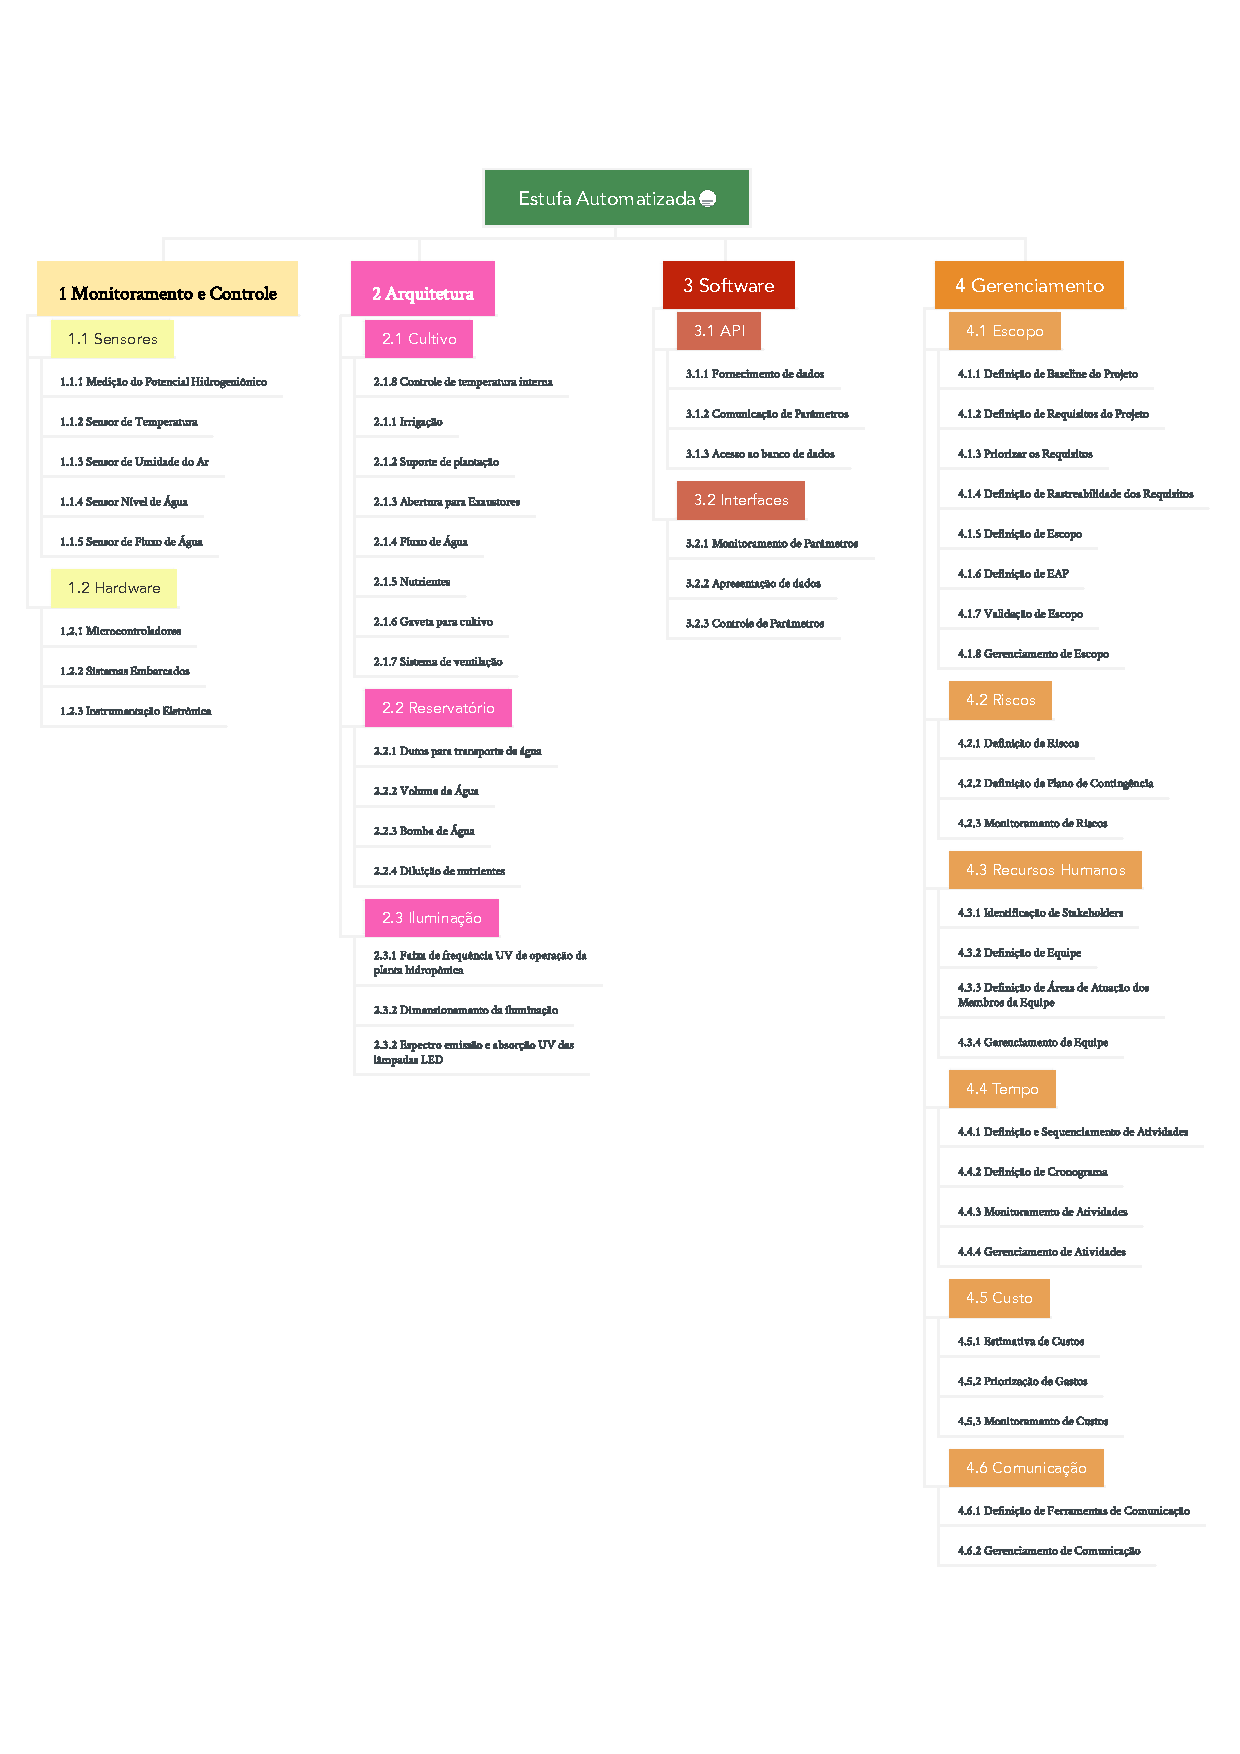
\includegraphics[width=15cm]{figuras/eap.pdf}
	\caption{EAP - estrutura analítica do projeto} \label{eap}
\end{figure}

\subsection{Plano de gerenciamento de tempo}

O gerenciamento do tempo se torna necessário no projeto pois desse modo será possível descrever os processos e atividades que deverão ser executadas do início ao fim do projeto, tendo em foco a garantia da execução das atividades nos prazos definidos previamente e que haja um controle cronológico da execução das atividades.

\subsubsection{Papeis e responsabilidades}

Os gerentes do projeto ficarão responsável pela avaliação de qualidade e melhoria contínua dos subsistemas do processo de integração e também pelo pleno funcionamento e testes dos subsistemas. Será feita uma validação com a equipe geral do projeto e em seguida a integração.

\subsubsection{Cronograma}

\begin{figure}[H]
	\centering
	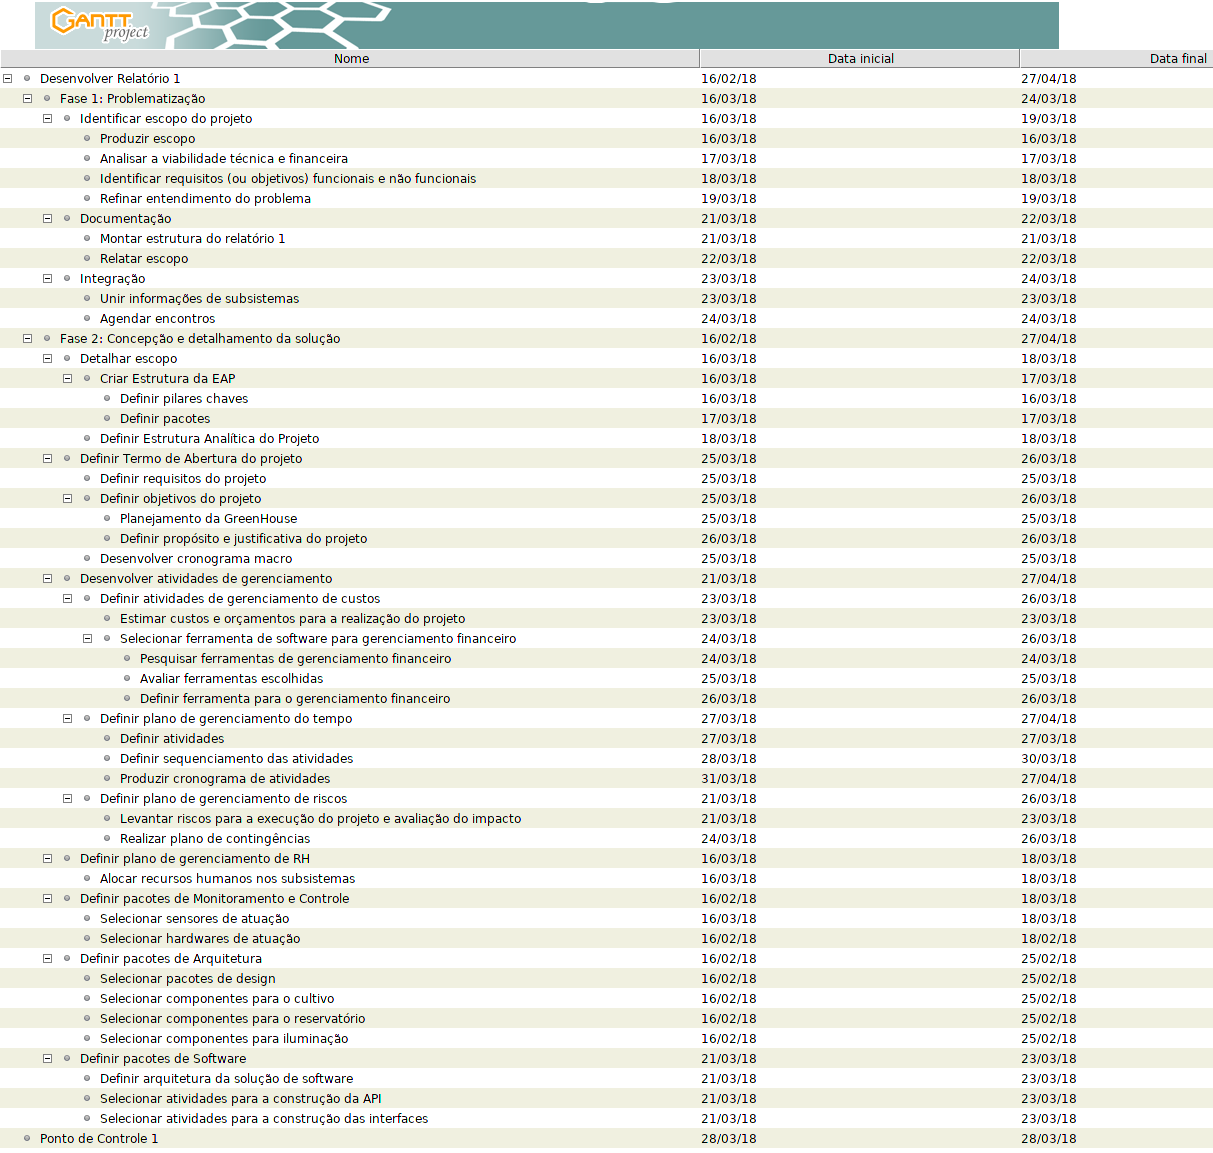
\includegraphics[width=16cm]{figuras/cronograma_1.png}
	\caption{Cronograma do projeto} \label{cronograma_1}
\end{figure}

\begin{figure}[H]
	\centering
	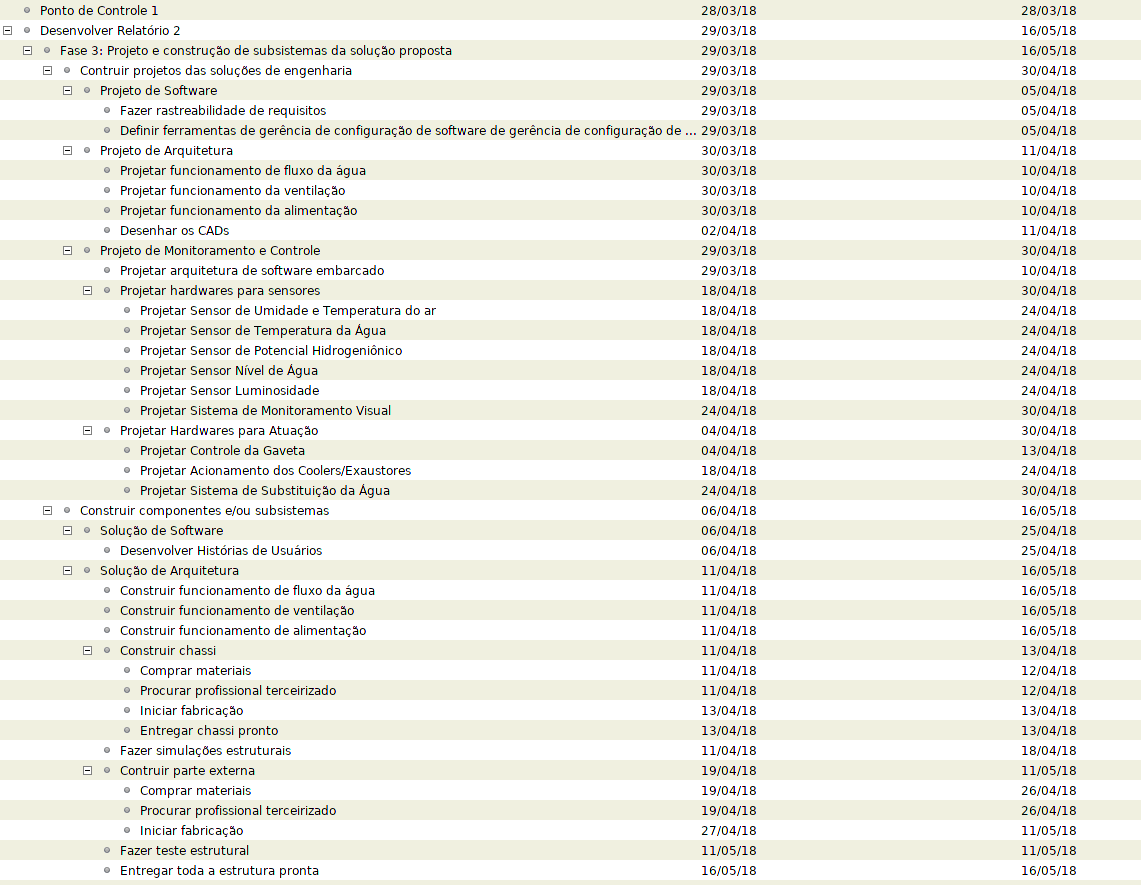
\includegraphics[width=16cm]{figuras/cronograma_2.png}
	\caption{Cronograma do projeto} \label{cronograma_2}
\end{figure}

\begin{figure}[H]
	\centering
	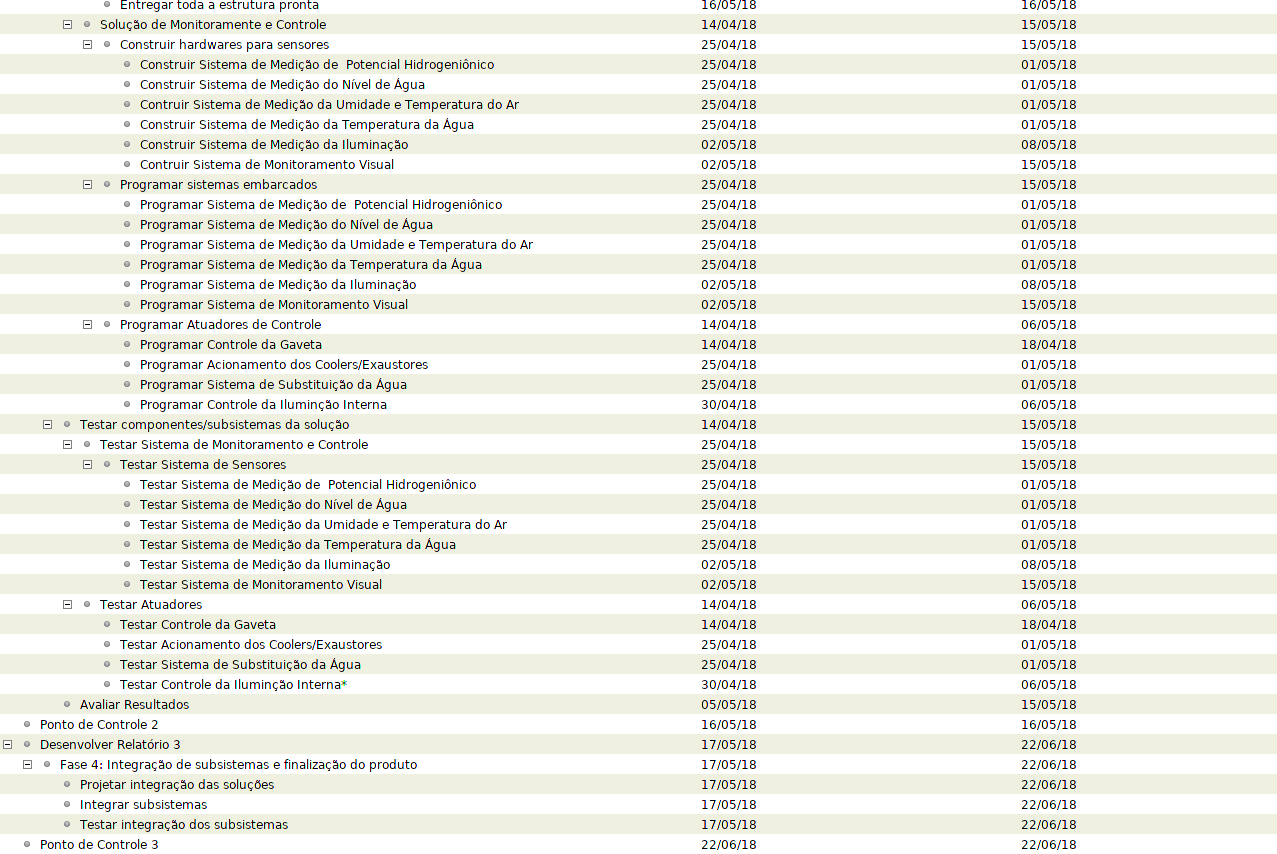
\includegraphics[width=16cm]{figuras/cronograma_3.png}
	\caption{Cronograma do projeto} \label{cronograma_2}
\end{figure}

\subsection{Plano de gerenciamento de comunicação}

Durante a execução do projeto, a comunicação do grupo será realizada por meio de duas formas principais: reuniões físicas, utilização de ferramentas de comunicação.

\subsubsection{Reuniões presenciais}

Serão realizadas reuniões presenciais entre os membros da equipe de projeto duas vezes por semana. Tais reuniões serão devidamente documentadas por meio de pautas, seguindo um modelo pré-estabelecido pela equipe.

\subsubsection{Ferramentas de comunicação}

Durante a execução do projeto, serão utilizadas ferramentas de comunicação e gerenciamento de projeto, tanto para permitir a fácil transmissão de informações entre os membros da equipe, quanto para o acompanhamento e monitoramento do trabalho. As ferramentas utilizadas são apresentadas a seguir:

\begin{itemize}
	\item Slack: Utilizada como principal meio de comunicação da equipe, a ferramenta Slack permite a criação de diversos canais dentro de um mesmo projeto. Estes canais serão utilizados para facilitar o gerenciamento das comunicações, havendo um canal específico para cada subárea do projeto, além de um canal geral. O Slack permite também a integração com diversas ferramentas de gerenciamento de projetos, tais como o Trello e bots.
	
	\item Trello: Para o gerenciamento e acompanhamento do projeto, será utilizado um board da ferramenta Trello, que permite a definição de tarefas a serem executadas. Por meio da criação de listas, é possível acompanhar o andamento do projeto. Tais listas evidenciam as atividades que se encontram no backlog, as que estão sendo executadas no momento, as que aguardam algum tipo de validação, entre outros estados de completude que a equipe julgar necessário evidenciar. Além disso, o Trello permite observar quem são os membros responsáveis pela execução de cada atividade.
	
	\item Geekbot: O Geekbot é uma ferramenta de questionários automatizados que podem ser enviados diariamente aos membros da equipe pela ferramenta Slack. A partir da definição de um questionário simples e de um canal para a postagem das respostas no Slack, é possível acompanhar as atividades diárias referentes ao projeto dos membros da equipe de forma individual, facilitando o gerenciamento de atividades. 
	
	\item Google Drive: Para o armazenamento e edição de documentos pertinentes ao projeto, será utilizada a ferramenta Google Drive. A partir dela, é possível que documentos e arquivos sejam compartilhados entre todos os membros da equipe de forma organizada e instantânea. Além disso, é possível a edição conjunta de documentos, o que facilita o desenvolvimento de artefatos necessários para o desenvolvimento do projeto.
	
\end{itemize}

\subsection{Plano de gerenciamento de riscos}

A probabilidade de ocorrência de um risco ou oportunidade é classificada em baixa, média e alta. De forma similar, o impacto de um risco ou oportunidade também é classificado como baixo, médio ou alto. Por fim, a prioridade de um risco ou oportunidade é uma relação entre sua probabilidade e seu impacto, e varia de 1 (baixa prioridade) a 3 (alta prioridade).

\begin{figure}[H]
	\centering
	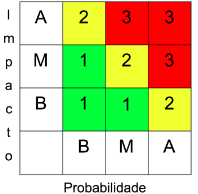
\includegraphics[width=4cm]{figuras/riscos.png}
	\caption{Riscos} 
	\label{Risco}
\end{figure}

\begin{table}[]	
	\centering
	\resizebox{\textwidth}{!}{%
	\begin{tabular}{|l|l|l|l|l|}
		\hline
		ID & Descrição do Risco & Probabilidade & Impacto & Prioridade \\ \hline
		1 & Mal funcionamento de sensores. & Baixa & Alto & 2 \\ \hline
		2 & Saída de um membro da equipe. & Alta & Médio & 3 \\ \hline
		3 & Demora na entrega de equipamentos adquiridos. & Média & Médio & 2 \\ \hline
		4 & Indisponibilidade dos membros do grupo. & Média & Médio & 2	 \\ \hline
		5 & Falha ou impossibilidade de comunicação entre hardware e software. & Baixa & Alto & 2 \\ \hline
		6 & Falta de verba para aquisição de equipamentos e material. & Média & Alto & 3 \\ \hline
		7 & Desinformação na equipe do projeto. & Média & Baixo & 1 \\ \hline
		8 & Aquisição de investimento para o projeto. & Baixa & Alto & 2 \\ \hline
			9 & Documentação inconsistente. & Média & Médio & 2 \\ \hline
			10 & Possíveis acidentes. & Baixa & Alto & 3 \\ \hline
	\end{tabular}%
}
	\caption{Tabela responsável por realizar o mapeamento da descrição de cada risco e seus impactos, probabilidades e prioridades.}
	\label{Riscos}
\end{table}

\begin{itemize}
	\item 1 - Mal funcionamento de sensores \\
	Possíveis consequências: prejuízo financeiro, atraso em determinada etapa de fabricação do produto; leitura errônea de medições. \\
	Ação: mitigar. Realizar pesquisa de mercado e adquirir sensores de marcas cuja qualidade é reconhecida; utilizar os sensores seguindo seus manuais ou guias de uso; realizar debug dos sensores.
	
	\item 2 - Saída de um membro da equipe \\
	Possíveis consequências: excesso  de trabalho sobre demais membros da equipe; atraso em determinadas etapas de fabricação do produto; aumento de despesas individuais. \\
	Ação: aceitar. A realocação de trabalho será pensada de acordo com o subsistema ao qual pertencia o membro sainte.
	
	\item 3 - Demora na entrega de equipamentos adquiridos \\
	Possíveis consequências:  atraso em determinada etapa de fabricação do produto. \\
	Ação: mitigar. Realizar pesquisa de mercado sobre a loja virtual na qual se planeja comprar; optar por tipo de envio mais rápido disponível, conforme necessidade; realizar pedidos tão logo se perceba a necessidade de determinado equipamento, mesmo que ainda se demore a utilizá-lo, e pesquisar em lojas próximas.
	
	\item 4 - Indisponibilidade de um membro do grupo \\
	Possíveis consequências: excesso de trabalho sobre os demais membros do grupo; atraso em determinadas etapas de fabricação do produto. \\
	Ação: mitigar. Sempre que possível, avisar com antecedência o período de indisponibilidade. Em caso de ausências prolongadas, exigir justificativa plausível, médica ou judicial.
	
	\item 5 - Falha ou impossibilidade de comunicação entre hardware e software \\
	Possíveis consequências: atraso em determinadas etapas de fabricação do produto. \\
	Ação: evitar. Adquirir equipamentos cuja compatibilidade com o software utilizado seja reconhecida. Garantir funcionamento de tecnologia Wi-Fi, Bluetooth ou outra tecnologia necessária.
	
	\item 6 - Falta de verba para aquisição de equipamentos e material \\ 
	Possíveis consequências: atraso em determinadas etapas de fabricação do produto; redução de escopo do produto. \\
	Ação: evitar. Gerenciar e monitorar custos do projeto ao longo de todo o seu ciclo de vida.
	
	\item 7 - Desinformação na equipe do projeto \\
	Possíveis consequências: atraso em determinadas etapas de fabricação do produto; retrabalho; gastos desnecessários. \\
	Ação: mitigar. Realizar reuniões informativas diárias. Documentar decisões e alterações em qualquer área de gerenciamento.
	
	\item 8 - Aquisição de investimento para o projeto \\
	Possíveis consequências: aumento de verba; possibilidade de comercialização tão logo ocorra a finalização do projeto. \\
	Ação: explorar. Realizar pesquisa de mercado, levantando possíveis áreas e entidades com potencial interesse no produto. Elaborar apresentação formal do produto.
	
	\item 9 - Documentação inconsistente \\
	Possíveis consequências: falha na comunicação entre membros da equipe; atraso em determinadas etapas da fabricação do produto; prejuízo financeiro; desentendimento por parte de terceiros em relação ao projeto. \\
	Ação: evitar. Validar todos os documentos escritos. Realizar controle e gerenciamento relativo a alterações.
	
	\item 10 - Possíveis acidentes \\
	Possíveis consequências: perda de um membro por um tempo determinado; perdas no orçamento; atraso na criação da estrutura. \\
	Ação: evitar. Utilizar os EPIs e EPCs necessários de acordo com as normas da ABNT; em casos de possíveis acidentes, trabalhar com a supervisão de um profissional.
	
	
\end{itemize}